\chapter{Architectural Viewpoint}
For this project we have chosen to make use of the \emph{4+1 view model}, where we have put most ephasis on the \emph{Logic}, \emph{Development} and \emph{Process} views.

    \section{Logic View}
    \textbf{Purpose:} In the Logic View we decompose the functional requirements into different classes and show the relationship between these requirements. This in order to showcase the functionality that the system provides to the end users.
    These classes supports showing the level of abstraction, encapsulation and inheritance.% in the system.
    The decomposition also helps identify elements that are shared across the system. 
    
    \noindent\textbf{Stakeholders:} Course staff, ATAM evaluators and Developers 
    
    \noindent\textbf{Form of description:} UML Class diagram.
    
    \section{Development view}
    \textbf{Purpose:} In the development view we illustrate how the different parts of the system looks a developers perspective. Different parts of the system is divided into layers. This view supports allocation of requirement
    and work to developers and also monitoring project progress.  
    
    \noindent\textbf{Stakeholders:} Course staff, ATAM evaluators and Developers
    

    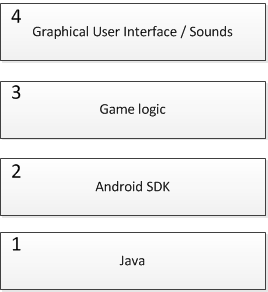
\includegraphics{DevelopmentView.png}
    
    \noindent\textbf{Form of description:} Architecture Layer Diagram. 
    
    \section{Process view}
    \noindent\textbf{Purpose:} In the process view we illustrate how different tasks are combined into the final product. In the process view we consider performance and availability requirements, and also system integrity and fault tolerance.
    The process view can specify which thread of control executes operations in the classes identified in the logic view. 
    
    \noindent\textbf{Stakeholders:} Users, Course staff, ATAM evaluators and Developers 
    
    \noindent\textbf{Form of description:} Graph?